
\begin{figure}[t]
  \centering
  \tikzstyle{b} = [rectangle, draw, fill=none, text centered, sharp corners, minimum height=3em, text width=2cm]
  \tikzstyle{l} = [draw, thick, ->]

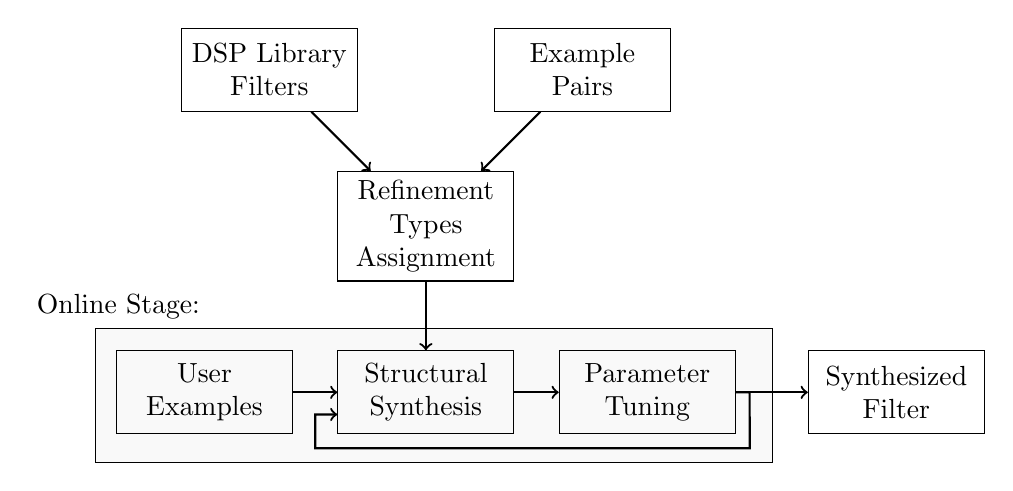
\begin{tikzpicture}[node distance = 8em, auto]
    % Place nodes
    \draw [fill=gray!05, opacity=1] (-4.2,-3) rectangle (4.4,-1.3);
    \node [b] (refty) {Refinement Types Assignment};
    \node [b, above left of=refty] (filters) {DSP Library Filters};
    \node [b, above right of=refty] (exs) {Example Pairs};
    \node [b, below of=refty, node distance=6em] (struct) {Structural \\ Synthesis};
    \node [b, left of=struct, node distance=8em] (examples) {User \\ Examples};
    \node [b, right of=struct, node distance=8em] (params) {Parameter Tuning};
    \node [b, right of=params, node distance=9em] (synth) {Synthesized Filter};
    \node [above left of=examples,node distance=4.4em] (online) {Online Stage:};

%Online Flow

    % Draw edges
    \path [l] (filters) -- (refty);
    \path [l] (exs) -- (refty);
    \path [l] (refty) -- (struct);
    \path [l] (examples) -- (struct);
    \path [l] (struct) -- (params);
    \draw [l] (params.east) -- ([xshift=0.5em]params.east) -- ([yshift=-0.5em,xshift=3.7em]params.south) -- ([yshift=-0.5em,xshift=-4em]struct.south) -- ([yshift=-0.8em,xshift=-0.8em]struct.west) -- ([yshift=-0.8em]struct.west);
    \path [l] (params) -- (synth);

\end{tikzpicture}
  \caption{Synthesis first assigns refinement types to the DSP filter in an offline stage, then uses a feedback loop to synthesize program structure and parameters based on user-provided examples.}
  \label{fig:high_level_overview}
\end{figure}




